\documentclass{beamer}
\usepackage{array}

\usetheme{Warsaw}
\usecolortheme{crane}

\setbeamertemplate{caption}{\raggedright\insertcaption\par}

%\setbeamertemplate{caption}[numbered]

\title[Cool Baking]{Bake: A Compiler for Cool}
\author{The Cake Whisperers: \\AJ, Melanie, Russell, Will}
\date{\today}

\begin{document}
%\maketitle{}
\frame{\titlepage}

\begin{frame}
  \frametitle{Development Style}

  \begin{itemize}
    \item Using Google Style Guide.
    \item Using CMake for building\footnotemark.
    \item Team communication via Slack.
    \item Using Git for version control.
    \item Rebase-based workflow.
    \item Working branch \texttt{dev} with ``stable'' branch \texttt{master}.
  \end{itemize}

  \begin{figure}
    \centering
    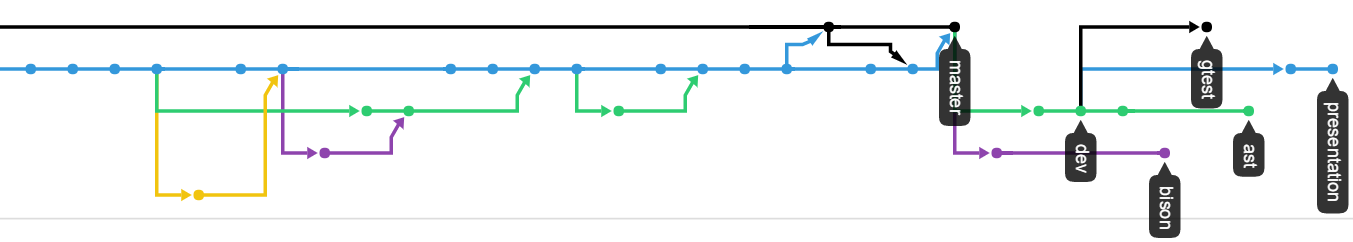
\includegraphics[width=\linewidth]{img/network}
  \end{figure}

  \footnotetext[1]{The source of many tears.}
\end{frame}

\begin{frame}
  \frametitle{Testing}

  \begin{itemize}
  \item Using CircleCI to test each commit automatically.
  \item Using Google Test as our testing framework.
  \item Kept in line by our Eggplant Overlord.
  \end{itemize}

  \begin{figure}
    \centering
    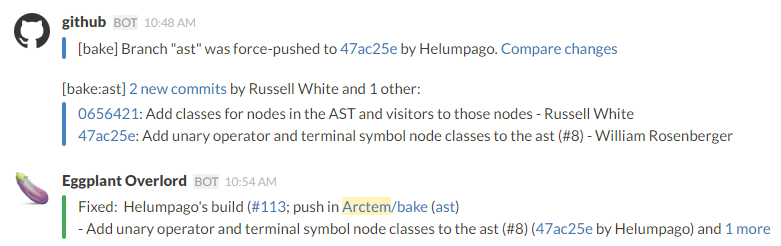
\includegraphics[width=\linewidth]{img/slack}
  \end{figure}

  \begin{figure}
    \centering
    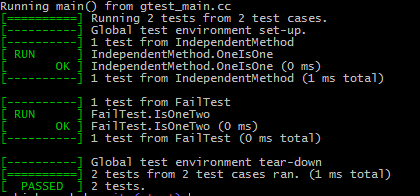
\includegraphics[width=0.5\linewidth]{img/test}
  \end{figure}
\end{frame}

\begin{frame}
  \frametitle{Flex}

  \begin{itemize}
  \item We made it work...yeah.
  \end{itemize}
\end{frame}

\begin{frame}
  \frametitle{Bison}

  \begin{itemize}
    \item After designing BISON we reconfigured Flex to tokenize what we needed.
    \item BISON workflow is very similar to the Cool Syntax Grammar.
    \item We decided to break up some of our syntax into further grammar
      productions for easy modification and readability.
    \item BISON is a work in progress throughout our AST creation.
  \end{itemize}
\end{frame}

\begin{frame}
  \frametitle{AST Design}

  \begin{columns}
    \column{0.5\linewidth}
    \begin{itemize}
      \item Each node represents an action taken by the program
      \item Terminals are the only nodes that contain actual values
      \item Non-terminals contain references to other nodes
      \item Each node defines getters/setters for its children
      \item Using the visitor design pattern
    \end{itemize}

    \column{0.5\linewidth}
    \begin{figure}
      \centering
      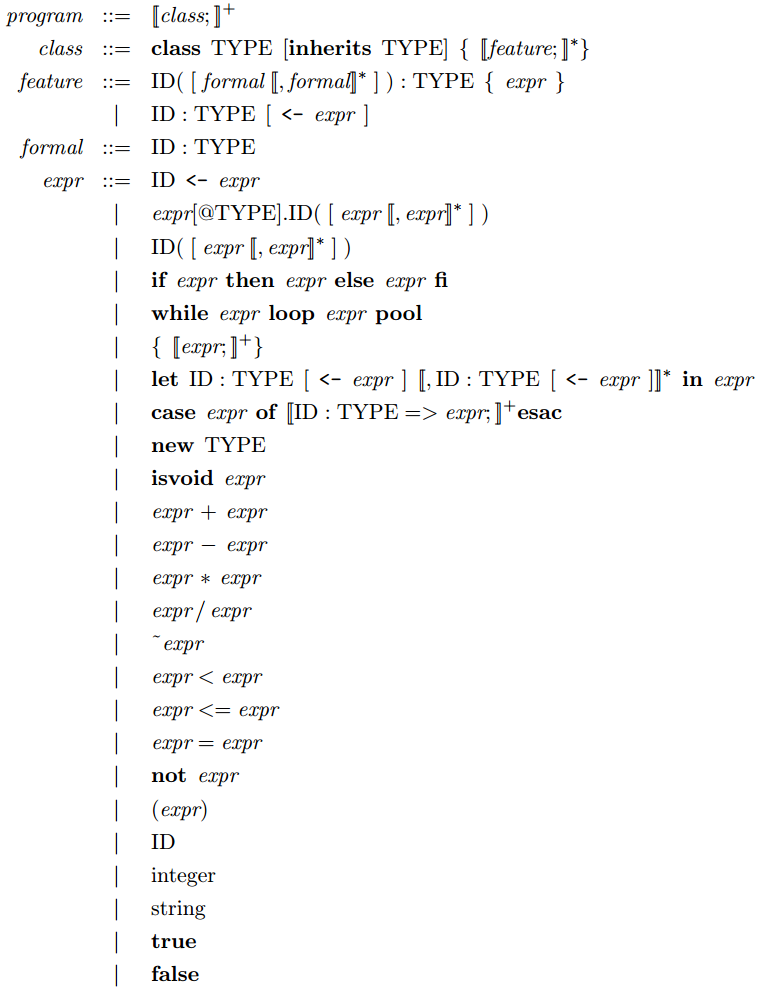
\includegraphics[width=\linewidth]{img/hierarchy}
    \end{figure}
  \end{columns}
\end{frame}

\end{document}
